\section{Introduction}

Deep learning has become the default approach for image classification tasks, with convolutional architectures and transfer learning making it feasible to build competitive models on modest datasets without training from scratch.
This assignment applies that toolkit to a dataset of Lego Minifigures scraped from brickset.com. The target is the \texttt{category} attribute, framing the problem as multiclass classification. Given the strong class imbalance, the label space is restricted to the top-$k$ most frequent categories rather than the full set. The pipeline compares several pretrained backbones, fine-tunes the selected one, and documents the architectural trade-offs and regularisation choices used to keep overfitting in check. Model behaviour is then probed with a confusion matrix and Grad-CAM to identify which regions of the image drive predictions, followed by a critical reflection on what the metrics and visualisations actually reveal about the model's reliability.

\section{Data description}
\subsection{Data sources}
The dataset consists of JPG images of individual minifigures. The figures themselves are visually uniform in pose and framing, but the background varies: most are shot on white, some on light brown, and a smaller subset includes a floor as background. When a figure wears a mask or helmet, the underlying head is typically shown as a smaller inset in the upper-right corner of the image.
Metadata is supplied in \texttt{minifigs.json}, with one entry per figure. The fields relevant to this assignment are:
\begin{itemize}
    \item \texttt{category}: heavily imbalanced, ranging from 3,522 objects in the largest class down to a single object in the smallest
    \item \texttt{year\_released}: spans 1975 to 2026
    \item \texttt{current\_value\_used} / \texttt{current\_value\_new}: strings formatted as either "\textasciitilde{}€4.21" or "Not known"
    \item \texttt{themes}: only 87 figures carry three or more theme labels.
\end{itemize}
The remaining fields (\texttt{id}, \texttt{name}, \texttt{link}, \texttt{year}, \texttt{img\_}\allowbreak\texttt{url}, \texttt{minifig\_}\allowbreak\texttt{number}, \texttt{subcategory}, \texttt{set\_}\allowbreak\texttt{id}, \texttt{character\_}\allowbreak\texttt{name}, and \texttt{img\_}\allowbreak\texttt{local\_}\allowbreak\texttt{path}) are not used for the classification task.

\subsection{Data structure}
The JPG files are not stored in the same order as the entries in the JSON file, so the first preprocessing step is to align each image with its corresponding metadata record (via \texttt{minifig\_number} / \texttt{img\_local\_path}) before any splitting or training can take place.

\section{Choice of modelling objective}
Of the three proposed candidate deep learning models, we decided to go forward with Multiclass classification. The multilabel formulation was discarded on the grounds of insufficient signal: only 87 objects carry three or more theme labels, leaving the multilabel structure too sparse to justify the added complexity. Regression was also set aside. Predicting the year of release was deemed too ambiguous to yield reliable visual features, and predicting the value is complicated by its string format. The analysis of this format would preclude the use of GRAD-CAM for visual explainability of the classifications. 

\section{Data preprocessing and assessment of top-$k$ category count and pre-trained backbone}
\subsection{Train/Validate/Test split}
We consecutively applied a stratified 70/15/15 split over the retained top-$k$ categories. Stratification was applied at the category level so that each subset preserves the global class distribution. This matters because the within-top-$k$ distribution is highly imbalanced (e.g. for the top-40 setup, the largest class is 65$\times$ the smallest class), and an unstratified split would magnify that imbalance in evaluation.
For the same reason, macro F1 was chosen as the evaluation metric. It averages F1 across classes with equal weight, so performance on small categories counts as much as performance on large ones. Plain accuracy would be dominated by the largest classes and would mask failures on the long tail.

\subsection{Top-$k$ category count}
The first two runs both used \texttt{MobileNetV2} as backbone from \texttt{keras.applications}, with a frozen ImageNet-pretrained backbone, balanced class weights, and an otherwise identical training procedure. The only variable was the label space: top-64 versus top-20. Macro F1 came in at 0.57 and 0.68 respectively, a gap of 0.11. Because architecture and training procedure were held constant, this gap is attributable cleanly to category count.
To balance informativeness against per-class sample size, $k=40$ was chosen for the main model. This retains 33\% of the original 122 categories while still implying a 65$\times$ imbalance between largest and smallest class (3,522-54 samples).
A possible alternative was to keep the top 40 and bin the remaining 82 categories into a single "Other" class. This was rejected: with more than two thirds of categories collapsed into one bucket, "Other" would dominate the loss and distort the macro F1, while training pressure would be diverted away from the categories that actually matter.

\subsection{Pre-trained backbone}
Backbones were compared on the top-20 setup rather than top-40, reusing the \texttt{MobileNetV2} run from 4.2 as the baseline. The run was compared to \texttt{EfficientNetV2S}, a heavier, more recent backbone demanding a higher resolution (384$\times$384 versus 224$\times$224 for \texttt{MobileNetV2}), also from \texttt{keras.applications}. Macro F1 moved from 0.68 to 0.70. The improvement is real but smaller than the top-$k$ gap, and since category count is held constant, the 0.02 reflects architecture alone: \texttt{EfficientNetV2S} extracts somewhat stronger features from this dataset.
\texttt{EfficientNetV2S} was selected for the main model. The comparison was run with a frozen base, so the 0.02 gain measures only the quality of the pretrained features feeding into the head. With partial fine-tuning of the upper layers (Section 6), the stronger backbone has more room to adapt and the gap is expected to widen.

\section{Data and preprocessing}
\subsection{Splits and resolution}
As mentioned before, we applied a stratified 70/15/15 split over the 40 retained categories. Images were loaded at 384$\times$384 through Keras's \texttt{ImageDataGenerator} with batch size 16.
No custom preprocessing of backgrounds or minifig framing was applied. Although backgrounds occasionally deviate from the standard white (light brown, floor scenes), the minifigures themselves are near-uniform in size and position within the frame, so a generic crop or background-removal pass risked introducing more noise than it removed. This decision was validated post-hoc via Grad-CAM (Section 8.2): the activation maps consistently focus on the minifigure body rather than the background, and for figures with an inset head in the upper-right corner, on the main figure rather than the inset.
The \texttt{rescale} parameter of \texttt{ImageDataGenerator} was deliberately left at \texttt{None} as \texttt{EfficientNetV2} includes a built-in normalisation layer.

\subsection{Augmentation}
Augmentation was applied to the training generator only, leaving the validation and test generators (\texttt{shuffle=False} on the latter) untouched so that evaluation runs on unaltered images. The training pipeline applied random rotations of up to 30$^\circ$, horizontal and vertical shifts of up to 20\%, brightness scaling in the [0.8, 1.2] range, horizontal flipping, and zooming up to 20\%, with nearest fill for any newly exposed pixels.

\subsection{Initial class weights}
To handle category imbalance, we computed balanced weights using the \texttt{compute\_}\allowbreak\texttt{class\_}\allowbreak\texttt{weight} function (with \texttt{class\_}\allowbreak\texttt{weight='balanced'}) from \texttt{sklearn}. Since macro F1 is our headline metric and weighs every class equally regardless of support, the loss function needs to treat them equally too. Without weighting, the optimiser would minimise loss most effectively by getting frequent classes right and effectively ignoring the rare ones. These weights were passed through the \texttt{class\_weight} argument of \texttt{model.fit} and applied in both Phase 1 and Phase 2. We return to them in Section 7.

\section{Model and two-phase training}
\subsection{Architecture}
The model uses \texttt{EfficientNetV2S} as the feature extractor, initialised with ImageNet weights. On top of the convolutional base we built a custom head as a \texttt{Sequential} stack: \texttt{GlobalAveragePooling2D} to collapse the spatial dimensions, then a \texttt{BatchNormalization} layer, a \texttt{Dense(512, relu)} for the task-specific projection, a \texttt{Dropout(0.4)} for regularisation, a second \texttt{BatchNormalization}, and a final \texttt{Dense(40, softmax)} for the multiclass output.

\subsection{Phase 1: head training}
In the first phase the entire \texttt{EfficientNetV2S} backbone was frozen (\texttt{base\_model.trainable = False}), so gradients flowed only into the new head. The model was compiled with the Adam optimizer at a learning rate of $10^{-3}$, a deliberately high starting point, since at this stage we are training only freshly initialised dense weights. The loss function was \texttt{categorical\_crossentropy} against the one-hot targets, and we tracked accuracy, Precision, and Recall alongside loss, relevant given the macro-F1 framing.

\subsection{Phase 2: partial fine-tuning}
The base model was unfrozen, after which we re-froze all but the last 100 layers, roughly the top fifth of \texttt{EfficientNetV2S}, which has 513 layers in total. The reasoning is standard transfer-learning logic: lower layers encode generic visual primitives (edges, textures, colour gradients) that ImageNet already learned well on a far larger dataset than ours, while upper layers encode dataset-specific abstractions that benefit from adaptation to Lego minifigures.
The model was recompiled with a learning rate of $10^{-5}$, two orders of magnitude below Phase 1. This is essential to avoid catastrophic forgetting, where large weight updates erase the useful pretrained features we are trying to preserve. The loss function, metrics and class weights were unchanged. 

\section{Initial evaluation and class-weight smoothing}
\subsection{Initial evaluation}
After the two-phase training, the model was evaluated on the held-out test set. Overall accuracy reached 60\%, with a macro F1 of 0.58, macro precision of 0.54, and macro recall of 0.73. Macro F1 is the metric we focus on: by weighting every class equally regardless of support, it ensures that strong performance on rare categories is not buried under the bulk of frequent ones.
The precision-recall gap is the most informative number here. Recall at 0.73 means the model successfully retrieves most relevant instances across classes, but precision at 0.54 means more than four in ten of its positive predictions are wrong. The pattern was concentrated in the smaller classes, where recall was often near-perfect and precision floored out, a signature of a classifier that has been pushed too hard toward minority classes.

\subsection{Square-root smoothing}
The cause traces back to the standard \texttt{class\_weight='balanced'} setting from Section 5.3, which assigns each class a weight inversely proportional to its frequency. For a top-40 distribution where the rarest class has 65$\times$ fewer samples than the most frequent, this produces extreme weight ratios. The optimiser responds rationally: it lowers the decision threshold for rare classes, accepting a flood of false positives in exchange for catching every true case.
The fix is to compress the weight range without changing its rank order. We applied a square-root transformation to the balanced weights, \texttt{np.sqrt(balanced\_weights)}, which preserves the principle that rare classes deserve more weight than frequent ones but pulls the most extreme weights toward the median. 
The best-validation-loss checkpoint from the two-phase run was then reloaded and the model recompiled with the smoothed weights at a learning rate of $10^{-6}$: one order of magnitude below Phase 2, since the goal is now a gentle re-balancing of an already fine-tuned model rather than further feature adaptation.

\subsection{Final evaluation}
Re-evaluating on the held-out test set after the smoothed-weight pass produced 62\% accuracy, with a macro F1 of 0.60, macro precision of 0.56, and macro recall of 0.73. Accuracy moved up two points, macro F1 gained 0.02, precision rose by 0.02, and recall held flat.
The recall stability is the most important read on these numbers. Compressing the weight range reduces the optimiser's incentive to overpredict rare classes, which would normally come at the cost of recall as the model becomes more conservative, but recall did not move. The precision gain therefore came from genuinely cleaner decisions rather than from trading away coverage. The F1 improvement is modest in absolute terms but consistent with the diagnosis in 7.1: the original problem was a precision deficit on rare classes, and that is precisely where the smoothing acted.

\section{Visual analysis}
\subsection{Confusion patterns}
To establish where the model goes wrong before asking why, we plot the test-set predictions as a 40$\times$40 confusion matrix (Figure \ref{fig:confusion_matrix}). The diagonal is strongest for the four largest classes (DUPLO, Town, Friends, and Star Wars) which is expected: more training data buys cleaner decision boundaries. 
The clearest structural pattern off the diagonal is the Town row, which spreads thinly across many columns: when a true Town minifigure is misclassified, it scatters across a wide range of themes rather than concentrating on any single confuser. This matches what Town actually is, a category of generic civilian minifigures without distinctive theme decals and the symmetric scatter into the Town column from other rows suggests it also functions as the model's default guess when no theme-specific cues are present. Beyond Town, off-diagonal mass concentrates around visually similar movie and franchise themes (Star Wars, Super Heroes, The LEGO NINJAGO Movie), where the figures genuinely share design language and additional training data on its own would not resolve the ambiguity. 

\begin{figure}[H]
    \centering
    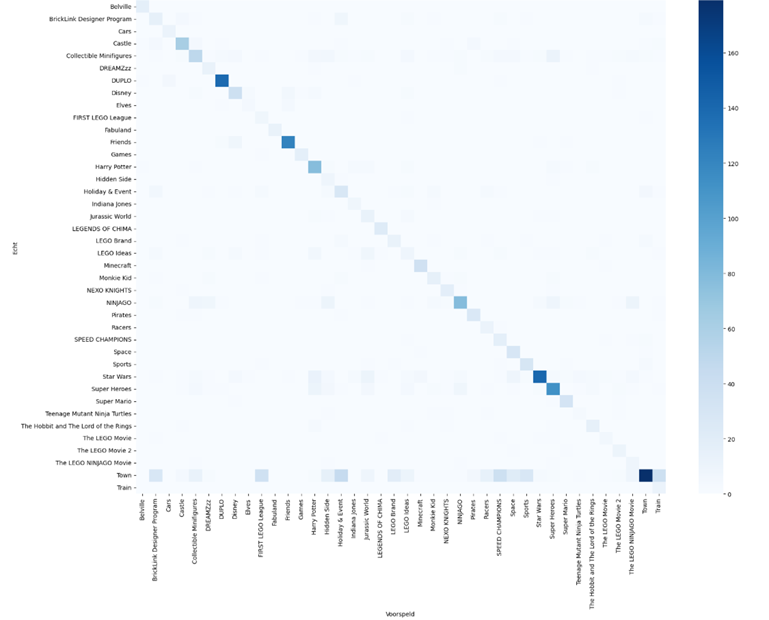
\includegraphics[width=\textwidth]{figures/A2_confusion_matrix.png}
    \caption{Confusion matrix for the top-40 Lego minifigure theme classification task.}
    \label{fig:confusion_matrix}
\end{figure}

\subsection{Grad-CAM}
\subsubsection{Set up}
The confusion matrix tells us which classes the model confuses; it does not tell us why. To inspect which regions of the image actually drive each prediction, we implemented Grad-CAM on the last convolutional layer of the \texttt{EfficientNetV2S} backbone (\texttt{top\_activation}). The procedure follows the standard formulation: we compute the gradient of the predicted class score with respect to the feature maps of that layer, pool those gradients spatially to obtain per-channel importance weights, and take a weighted sum of the feature maps using those weights. A ReLU and per-image normalisation produce a heatmap in [0, 1] indicating where attention concentrated for the chosen prediction.
For visualisation, we applied a 60th-percentile threshold to the heatmap to suppress low-attention regions before colouring, used the \texttt{inferno} colormap on the surviving values, and blended the result into the original image at a 0.55 / 0.7 ratio (heatmap / image). We ran the visualiser on 10 random test images, with each row showing the original, the overlay, and a summary block stating the predicted class, confidence, and whether the prediction was correct.

\subsubsection{Observations}
For correctly classified high-confidence cases, attention concentrates tightly on class-distinctive decals. On the Star Wars Darth Vader figure (97.5\% confidence) the heatmap locks onto the chest control panel and helmet. On the DUPLO firefighter (99.5\%) attention is on the helmet badge and the torso radio, both characteristic DUPLO printed elements. These are the cases the macro-F1 number is built on: the model has learned the right cues for the well-represented themes.
The more informative cases sit at the lower-confidence end. The Town civilian, correctly classified at 48.2\%, shows diffuse attention spread across the head and shoulders without any single cue dominating, consistent with a figure that simply carries no theme-specific decals to anchor on. A similar pattern appears for the Super Heroes Hulk (48.5\%), where diffuse torso attention reflects the fact that the Hulk's oversized non-standard proportions sit far outside the Super Heroes figures the model trained on. The confidence calibration is doing useful work here: low-confidence correct predictions correspond to genuinely ambiguous inputs, not random underconfidence.
The misclassification example illustrates the limit of what additional training can fix. A NINJAGO figure was predicted as Monkie Kid at 86.9\% confidence, with the heatmap focused on its head. The attention is on the right region but draws the wrong conclusion, because that visual signature exists in both themes. The model is reading the image correctly; the label boundary is what's underdefined. The off-diagonal bleed between visually similar themes in the confusion matrix reflects the same underlying problem.

\begin{figure}[H]
    \centering
    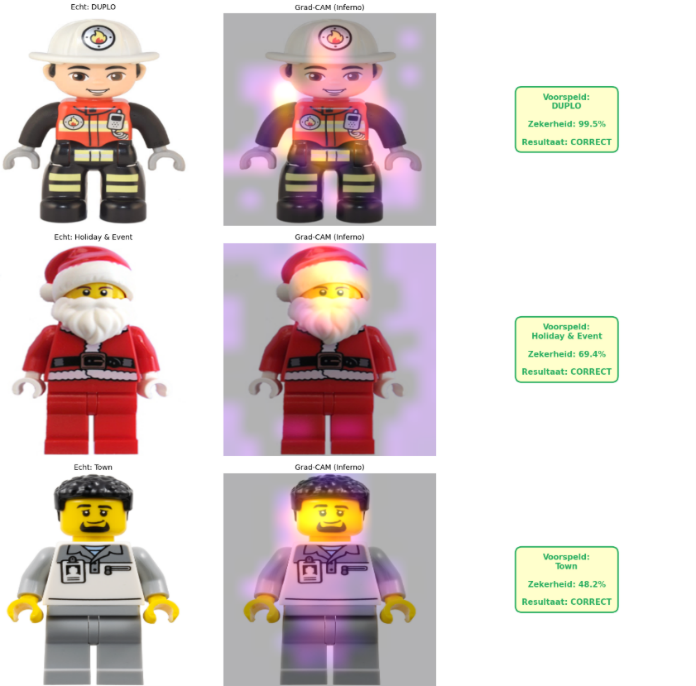
\includegraphics[width=0.85\textwidth]{figures/A2_GRADCAM1.png}
    \caption{Grad-CAM: High-confidence correct classification (Star Wars Darth Vader).}
\end{figure}

\begin{figure}[H]
    \centering
    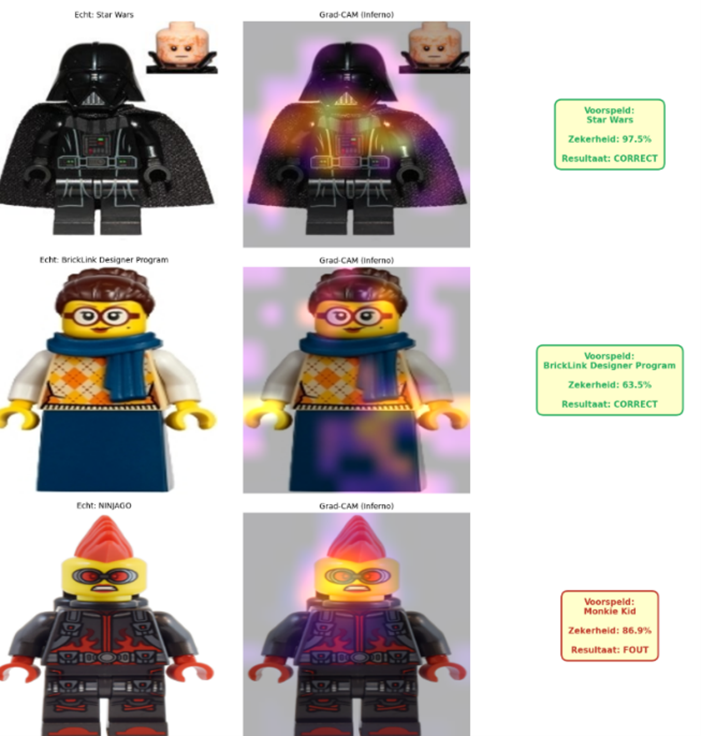
\includegraphics[width=0.85\textwidth]{figures/A2_GRADCAM2.png}
    \caption{Grad-CAM: Low-confidence correct prediction (Town civilian).}
\end{figure}

\begin{figure}[H]
    \centering
    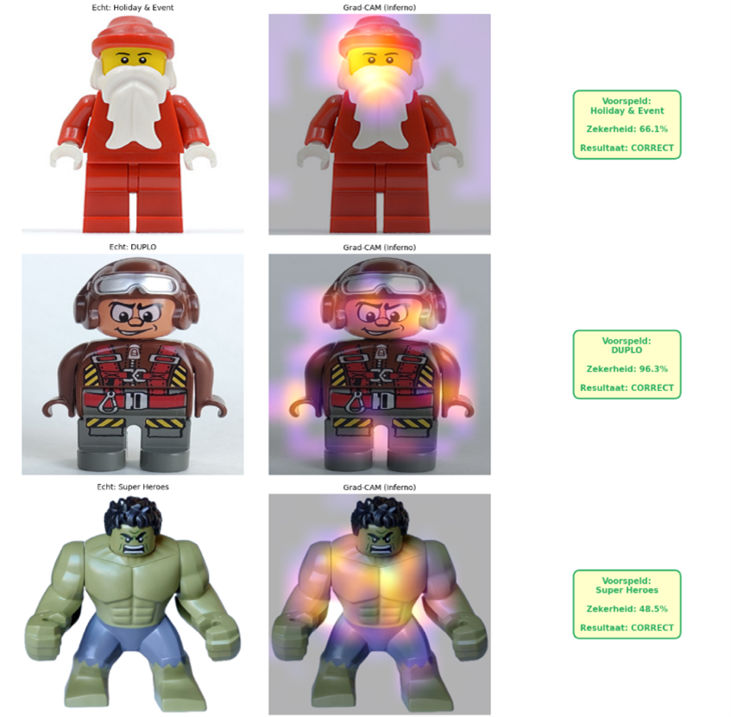
\includegraphics[width=0.85\textwidth]{figures/A2_GRADCAM3.png}
    \caption{Grad-CAM: Misclassification due to visual similarity (NINJAGO vs Monkie Kid).}
    \label{fig:gradcam}
\end{figure}

\section{Conclusion}
We arrived at a final macro F1 of 0.60 (62\% accuracy) on the top-40 test set, using \texttt{EfficientNetV2S} with a partially fine-tuned backbone, a custom head, and square-root-smoothed class weights. The three preliminary runs in Section 4 framed this as a defensible operating point: trimming the long tail did most of the heavy lifting on macro F1, while the backbone upgrade contributed a smaller but real margin on top. $k=40$ captures most of the category-count gain without trimming so aggressively that the task loses breadth, and \texttt{EfficientNetV2S} was retained on the expectation, borne out by the final result, that fine-tuning would extend its frozen-base advantage.
The biggest single in-training contributor was the class-weight smoothing in Section 7.2. The standard \texttt{class\_weight='balanced'} setting, which we initially treated as a sensible default, was in fact actively distorting the optimisation by depressing precision on rare classes. Reducing the weight range with a square-root transform, then applying a brief 3-epoch correction at a $10^{-6}$ learning rate, recovered roughly two points of macro F1 without forfeiting recall. Diagnostic refinement of an existing default outperformed any further architectural change we could plausibly have made within the time available, a useful lesson in where the marginal returns actually sit.
We also believe that further gains from this point are unlikely to be cheap. The remaining error mass concentrates in two places, both visible in Section 8: classes with limited training data and no distinctive visual cues (Town being the clearest case, where Grad-CAM showed diffuse attention because there is no theme-specific decal to anchor on), and clusters of themes that share design language so closely that the model attends to the right region but draws the wrong conclusion (the NINJAGO--Monkie Kid case being typical). Neither problem yields to backbone choice or hyperparameter sweeps. More data per rare class would help directly with the first, but is outside the scope of the assignment. A hierarchical approach, predicting a coarse theme cluster first, then a subtheme conditional on that, might reduce the precision penalty on the second, since classification within a cluster could focus on discriminating features rather than competing against 39 unrelated alternatives. Either of these would be a substantive next step rather than a tuning exercise, and we judge that the current result is a reasonable place to stop.
